\section{Messablauf}
\label{sec:Messablauf}

Für die Experimente wurde aus Kostengründen Nähgarn verwendet mit einem Durchmesser $D = 0,25~\si{\milli\metre}$ verwendet. Daraus ergibt sich nach \autoref{eq:achsenskalierungsfaktor} ein Skalierungsfaktor von $K_{xy} = 4$.Das zu wickelnde Medium (Faden, Draht, etc.) wird dann durch das Spannsystem und die Maschine eingeführt und am Spulenkörper befestigt. Die Maschine wird, mittels Commandlinebefehlen im Userinterface (UI), an ihre Startposition gefahren. Danach wird der Befehl zum Start des Kalibrationsscriptes gegeben, woraufhin das Programm einen zum tarieren der Wägezelle, sowie zum Messen eines Referenzgewichtes, auffordert. Zur Messung des Referenzgewichtes wird ein Smartphone an die eine Seite des Drahtes gebunden und die andere Seite fixiert. Da die Wägezelle so auf das doppelte Gewicht des Smartphones kalibriert wird, gilt für die ab nun, an der Wägezelle gemessenen Werte, $F_{WZ} = F_T$. Da sich in zuvor durchgeführten Tests gezeigt hat, dass die Wägezelle, hinsichtlich relativer Kraftänderungen, wiederholbare Ergebnisse produziert, bei Kalibration mit dem selben Gewicht, die absoluten Werte aber teils stark schwanken, wurde die Kalibration mittels Referenzgewicht nur einmal vor der Messserie durchgeführt. Da für unser Experiment das Augenmerk auf dem relativen Änderungen der Drahtspannung liegt, wurden die möglichen Absolutwertänderungen (z.B. Temperaturdrift) vernachlässigt, auch da eine erneute Kalibration ein Öffnen des Spannsystems voraussetzt, was zu weitaus schwerwiegenderen Problemen mit der Wiederholgenauigkeit führen würde.
Danach können die Befehl zur Durchführung unterschiedlicher Wickeloperationen gesendet werden. Es wird eine halbe Testlage gewickelt um zu sehen ob der Skalierungsfaktor stimmt und wenn nötig nachgestellt und erneut getestet (siehe \autoref{fig:wicklung_quader_einlagig}). Für unseren Draht ergab sich somit ein Skalierungsfaktor von $K_{xy} = 3$, mit $C = 0,75$. 
\begin{figure}[H]
    \centering
    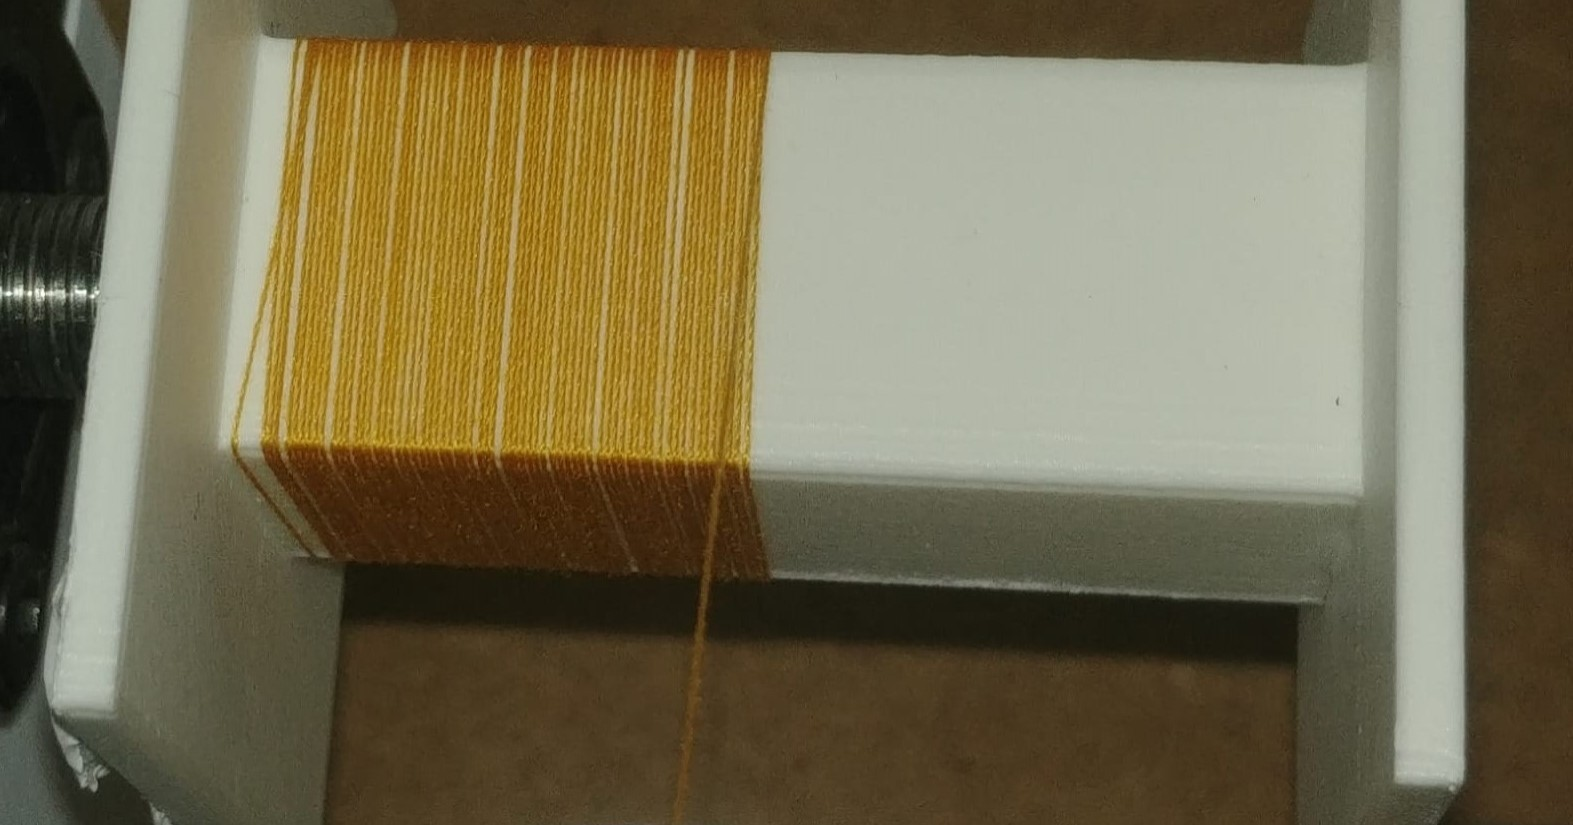
\includegraphics[width=0.6\textwidth]{./einlagenwickelung_quader.jpeg}
    \caption{Einlagige Wicklung von Nähgarn ($D = 0,25~\si{\milli\metre}$) auf Zylinder mit quaderförmigen Querschnitt ($s=20~\si{\milli\metre}$). Skalierungsfaktor $K_{xy} = 3$, Korrekturfaktor $C = 0,75$.}
    \label{fig:wicklung_quader_einlagig}
\end{figure}
Danach wird die  Messdatenübertragung per UI gestartet, wodurch die Übertragung der Messwerte über die Serielleschnittstelle beginnt. Bis zur Beendigung der Messung durch einen Commandlinebefehlen werden kontinuierlich Messdaten an den Computer übertragen. Für den genauen technischen Ablauf der Messung, siehe \autoref{sec:Messschleife}. 



